% ============================================================================
% PAQ-KV — AAAI-27 submission draft, distilled from paq_living.tex (2026-07-17).
% Every number is taken verbatim from the living document; nothing re-derived.
% Build: ./tectonic -X compile paq_aaai.tex
% ============================================================================
\documentclass[letterpaper]{article} % DO NOT CHANGE THIS
% ---------------------------------------------------------------------------
% LOCAL BUILD SHIM (this block only; the style file itself is untouched):
% the host has no pdflatex, so this draft is built with tectonic (XeTeX-based).
% aaai2027.sty's engine guard (\RequirePDFTeX) is neutralized ONLY when the
% engine is not pdfTeX. Under the official pdflatex build this block is inert
% and the guard runs as shipped. Remove the shim for the actual submission.
\usepackage{iftex}
\ifPDFTeX\else\let\RequirePDFTeX\relax\fi
% ---------------------------------------------------------------------------
\usepackage[submission]{aaai2027}  % DO NOT CHANGE THIS
\usepackage[hyphens]{url}  % DO NOT CHANGE THIS
\usepackage{graphicx} % DO NOT CHANGE THIS
\urlstyle{rm} % DO NOT CHANGE THIS
\def\UrlFont{\rm}  % DO NOT CHANGE THIS
\usepackage{natbib}  % DO NOT CHANGE THIS AND DO NOT ADD ANY OPTIONS TO IT
\usepackage{caption} % DO NOT CHANGE THIS AND DO NOT ADD ANY OPTIONS TO IT
\frenchspacing  % DO NOT CHANGE THIS
\usepackage{algorithm}
\usepackage{algorithmic}
\usepackage{booktabs}
\usepackage{multirow}
\usepackage{amsmath}
\usepackage{amssymb}

\pdfinfo{
/TemplateVersion (2027.1)
}

\setcounter{secnumdepth}{2}

\graphicspath{{figures/}}

\newcommand{\paq}{\textsc{PAQ}}
\newcommand{\paqt}{\textsc{PAQ-T}}
\newcommand{\paqc}{\textsc{PAQ-KV}}
\newcommand{\lb}{\mathrm{LB}_{95}}

\title{Prefill Once, Ask Many: Training-Free Reversible Below-Page KV Selection\\for Multi-Query Long-Document Visual Question Answering}
\author{
    Anonymous submission
}
\affiliations{
    Anonymous submission
}

\begin{document}

\maketitle

\begin{abstract}
Real document-VQA workloads are multi-query: one long document is prefilled once and asked many different questions. Standard KV-cache eviction commits to a single compressed context and reuses it for every question. We present \paqc{} (``prefill once, ask many''), a training-free, query-conditioned, \emph{reversible} below-page KV-selection method for a frozen vision--language reader: the document is prefilled once into the reader's KV cache and retained; per query, the reader's own question-to-content attention re-selects 64-token, page-aligned KV blocks, and the answer is decoded under a restricted-attention 4D mask over the intact cache---no re-read, no gathering, no second model, no index. The mechanistic contribution is \emph{reversibility}: per-query re-selection beats the identical scorer committed once on both benchmark cells (isolation contrast $+0.264$, $\lb=+0.187$ under a clean-cache re-run; block-level replication $+0.379$, $\lb=+0.273$). At a nominal 5\% decode-attention budget, \paqc{} beats ColQwen2, a state-of-the-art trained visual retriever, on MMLongBench-Doc ($0.404$ vs.\ $0.325$; $+0.079$, document-clustered $\lb=+0.041$; 80 documents / 444 queries), while \emph{matching} the gold-page oracle at that budget ($-0.026$, CI straddles zero) and matching full context. The result is adversarially audited: selection is query-dependent, query-specific (a wrong-question control collapses it, ruling out leakage), reversible, and below-page granularity beats page-level. On LongDocURL, \paqc{} matches but does not beat the retriever ($+0.019$, $\lb=-0.019$); we characterize why: only ${\approx}10\%$ of queries are selection-capturable and ${\approx}41\%$ fail even on native-resolution gold pages---a reader-conversion wall, not a selection wall. Two attempted selector upgrades (an externally learned per-head mixture; a sharp expert-head scorer) failed pre-registered gates and are reported as negatives. All results are development-pin evidence; a sealed held-out set is reserved for a single final evaluation.
\end{abstract}

\section{Introduction}\label{sec:intro}

Long-context vision--language models (VLMs) can read an entire multi-page document, but they pay for every page on every question. The standard efficiency response, inherited from single-query text benchmarks, is to \emph{evict}: keep a compact subset of the KV cache and decode against it \citep{li2024snapkv,zhang2023h2o,chen2024fastv,wan2024lookm,kim2025kvzip}. Eviction is a single, irreversible commitment: whatever subset is kept must serve every future question about that document.

Document assistants, however, are not asked one question. The two long-document VQA benchmarks we use are natively multi-query: grouping their 64K splits by source document, MMLongBench-Doc \citep{ma2024mmlongbench} averages ${\approx}6.97$ questions per document and LongDocURL \citep{deng2025longdocurl} ${\approx}3.6$; inside our pinned evaluation subsets the averages are 5.50 and 5.79 gold-bearing questions per document. Different questions need different evidence, so a subset committed for question~1 is \emph{stale} for question~5.

This paper asks: at a matched budget on long multimodal documents, does per-query \emph{re-selection} of context beat a \emph{commit-once} selection---and can a training-free, reader-internal selector compete with a dedicated trained retriever? Our answer is \paqc{}: prefill the full document \emph{once} into the KV cache of a frozen reader (Qwen3-VL-8B; \citealp{qwen3vl2025}) and retain it; per query, re-select the most relevant 64-token, below-page KV blocks with the reader's own question$\to$content attention; decode under a restricted-attention 4D mask over the retained full-context cache. Nothing is discarded and nothing is gathered (M-RoPE positions are untouched), so a selection is a \emph{view}, not a commitment: the next question re-selects from the same intact cache.

\paragraph{Contributions.}
\begin{itemize}
\item \textbf{Reversibility as the tested mechanism.} Under a pre-registered two-comparator isolation gate, per-query re-selection beats the identical scorer committed once on both cells (confirmatory run, 903 queries, 80 documents per cell, document-clustered inference: $+0.257$/$+0.163$ per cell) and beats a strong gold-informed static subset ($+0.108$/$+0.104$). The contrast survives a clean-cache re-run after an infrastructure fix ($+0.264$, $\lb=+0.187$), reappears at block level ($+0.379$, $\lb=+0.273$), and the same fresh-over-stale collapse holds for a retrieval scorer.
\item \textbf{\paqc{}, a training-free reversible below-page KV-selection method}: one prefill, per-query attention-guided block re-selection, and masked decode over the intact cache---no second model, no index, no re-read, and an exactness audit showing the mask machinery reproduces native decoding bit-consistently (zero mask-specific argmax changes).
\item \textbf{A powered, adversarially audited beat over a trained retriever.} On MMLongBench-Doc, \paqc{} at a nominal 5\% decode-attention budget scores $0.404$ vs.\ ColQwen2 $0.325$ at the matched budget ($+0.079$, document-clustered $\lb=+0.041$; 80 documents / 444 queries), while \emph{matching} the gold-page oracle at that budget ($-0.026$, CI straddles zero) and full context ($+0.009$, n.s.). The mechanism audit shows selection is query-dependent, query-specific (a wrong-question control collapses accuracy, ruling out leakage), reversible, and finer than pages by a significant margin.
\item \textbf{An honest, characterized limitation and two gated negatives.} On LongDocURL \paqc{} matches but does not beat ColQwen2 ($+0.019$, $\lb=-0.019$); we show the cell is mostly reader-conversion-bound rather than selection-bound. An externally learned per-head selection mixture (STOP) and a sharp expert-head block scorer (NO-GO) both failed pre-registered gates and are reported at full prominence.
\end{itemize}

\paragraph{Evidence status.} Every number in this paper is a development-pin result on an 80-document-per-cell pin; a sealed, disjoint held-out set (73/45 documents) is reserved for a single one-touch final evaluation that has not been run. We state this scope wherever it binds.

\section{Related Work}\label{sec:related}

\paragraph{Page-level attention selection.} CAPS \citep{zhu2026caps} publishes attention-based \emph{page} selection on our exact benchmarks: a scoring VLM's final-token$\to$page attention at one expert (layer, head), lightly calibrated off-benchmark, beats ColPali-pipeline retrieval. We state plainly that the ``reader-attention selects pages'' method is CAPS's. \paqc{} differs on the axes CAPS itself names as open: it operates \emph{below} page granularity, it is \emph{reversible} over one retained prefill rather than re-forwarding every page per query (CAPS reports 11.25\,s/query and concedes the multi-query regime to embedding methods), and it decodes directly from the masked cache with no re-read.

\paragraph{Visual document retrieval.} ColPali/ColQwen2 \citep{faysse2025colpali} embed pages once and re-rank per query; M3DocRAG \citep{cho2024m3docrag} and successors build pipelines on such retrievers; page-selection-then-read itself long predates this line \citep{mpdocvqa2024}. A published oracle analysis on MMLongBench \citep{hybridretriever2026} mirrors our own complementarity findings. ColQwen2 is the strong deployable baseline we compare against throughout.

\paragraph{KV compression and eviction.} SnapKV \citep{li2024snapkv}, H2O \citep{zhang2023h2o}, FastV \citep{chen2024fastv}, LOOK-M \citep{wan2024lookm}, and KVzip \citep{kim2025kvzip} commit a compressed cache once. Quest \citep{tang2024quest} shows query-aware selection beats query-agnostic eviction at tight budgets in single-query text---motivation for, but not evidence of, our multi-query claims. SparseVILA \citep{sparsevila2025} combines prefill pruning with decode-time retrieval but prunes irreversibly; Kamera \citep{kamera2026} shows the multi-query KV-reuse serving regime is becoming practically real.

\paragraph{Region-level and attention-guided neighborhood.} Region- and crop-level document methods are active: RegionRAG \citep{regionrag2025} (trained retriever-side crops), Snappy \citep{snappy2025} (patch-to-OCR-box localization), AGREE \citep{agree2025} (reader attention distilled into a trained retriever), agentic crop/zoom loops \citep{vragrl2025,docvstar2026}, and training-free single-image cropping \citep{vicrop2025,focus2025}; attention-based reranking precedents exist in text \citep{chen2025icr,wu2025qrhead}, and MMDocIR \citep{mmdocir2025} supplies layout-level labels. Our search did not identify prior work in the exact combined cell---reader-internal attention as the runtime below-page selector, end-to-end QA at matched budget against page-level retrieval, on long multi-query documents---which we offer as a provisional literature-map claim, not proof of novelty.

\section{Method: \paqc{}}\label{sec:method}

\subsection{Setting}
One long visual document, consumed as page images (no OCR), is read by a frozen VLM and will be asked $k$ questions (5.5--5.8 gold-bearing per document in our pins). The document is prefilled \textbf{once} at the same rendering the full-context arm uses ($\le$64K tokens) and the KV cache is \emph{retained}: never evicted, never physically compressed, never gathered. The cache plays the role a multi-vector index plays for a retriever---except it is the reader's own working memory, so retrieval and reading share one representation and one model.

\subsection{Per Query: Preview, Re-Select, Masked Decode}
\begin{enumerate}
\item \textbf{Preview (score).} The tokenized question is forwarded over the retained cache---with the cache crop-restored afterwards, so queries never contaminate one another (\S\ref{sec:integrity})---and the question rows' attention over context positions is aggregated into scores over \textbf{64-token, page-aligned KV blocks}: fine enough to isolate a table row, a figure caption, or a paragraph; coarse enough for the scores to be stable.
\item \textbf{Re-select.} Keep the top-scoring blocks at a \textbf{nominal 5\% decode-attention budget}. The terminology is deliberate: the kept blocks' K/V were computed with full-document context during the prefill (the standard claim semantics of the Quest/SnapKV method class), so this is a decode-attention budget, not a matched-token prefill comparison; the realized attended fraction on the executed screen is ${\approx}5.9$--$6.0\%$ of context and is always reported. The matched quantity against ColQwen2 is the evidence budget (5\% of pages vs.\ 5\% of context) at identical reader and scorer.
\item \textbf{Masked decode.} The answer is generated while attending only to the selected blocks plus a small \textbf{always-keep set} (the BOS/system/template scaffold, the question itself, and previously generated tokens), enforced by a \textbf{4D additive attention mask} (batch, head, query row, key) over the retained cache. \textbf{No gathering}: the K/V tensors stay at their original positions, so every M-RoPE rotary index is exactly the model's own---the failure mode that makes physical cache-gathering treacherous for VLMs is sidestepped entirely. No re-read, no re-render, no second model.
\end{enumerate}
Algorithm~\ref{alg:paqc} gives the loop; Figure~\ref{fig:paqkvloop} shows it schematically and Figure~\ref{fig:paqkvmask} the mask machinery. Attention is captured by OOM-safe per-layer forward hooks that reduce each layer's attention tensor immediately and discard it, so peak memory is one layer's attention (the naive all-layers path OOMs at long contexts).

\begin{figure}[t]
\centering
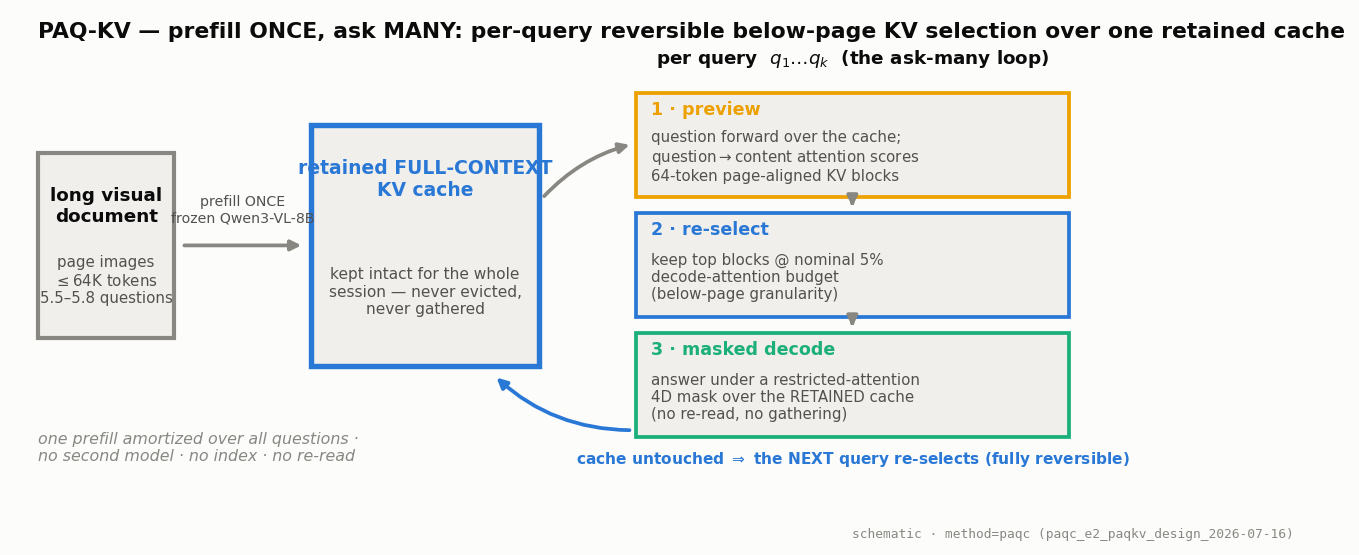
\includegraphics[width=\columnwidth]{fig_h_paqkv_loop_light.png}
\caption{The \paqc{} loop. The document is prefilled once into the frozen reader's KV cache, which is retained intact for the whole session. Each query runs the same three steps---attention preview, block re-selection, masked decode---against that one cache. No second model, no index, no full-resolution re-read; the cache is never modified, so selection is reversible by construction.}
\label{fig:paqkvloop}
\end{figure}

\begin{figure*}[t]
\centering
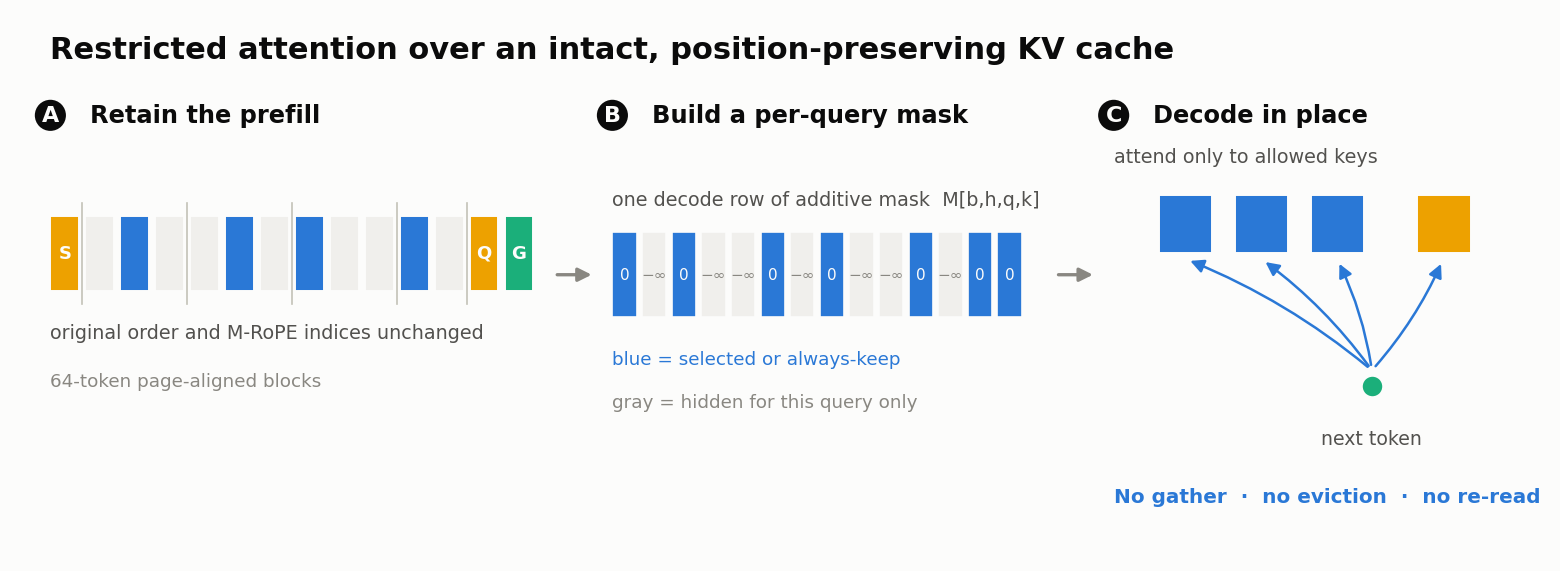
\includegraphics[width=0.92\textwidth]{fig_i_paqkv_mask_light.png}
\caption{The mechanism. The retained cache is a strip of K/V at their original positions: scaffold, page content in 64-token page-aligned blocks, question, generated tokens. The 4D additive mask lets decode rows attend only to the per-query selected blocks plus the always-keep set; everything else is masked \emph{for this query only}---it stays in the cache and remains selectable by the next query. Because nothing is gathered, the M-RoPE position machinery is untouched, and an all-true mask provably reproduces the native decode (identity audit: zero mask-specific argmax changes).}
\label{fig:paqkvmask}
\end{figure*}

\begin{algorithm}[t]
\caption{\paqc{}: per-query reversible below-page KV-block selection with a 4D restricted-attention mask}
\label{alg:paqc}
\begin{algorithmic}[1]
\REQUIRE document pages rendered as in the full-context arm ($\le$64K tokens); queries $q_1,\ldots,q_k$; nominal budget $b=5\%$; frozen VLM
\STATE prefill the document once; retain the full KV cache $C$ (context length $n_{\mathrm{ctx}}$); record page-aligned 64-token block spans $B_1,\ldots,B_m$ and the always-keep scaffold set $A$
\FOR{each query $q_j$}
\STATE forward the tokenized question over $C$; capture question$\to$context attention via per-layer hooks; \textbf{crop} $C$ back to $n_{\mathrm{ctx}}$
\STATE $\mathrm{score}(B_i) \gets$ aggregated question-row attention mass on block $B_i$'s positions
\STATE $S_j \gets$ top blocks by score at the nominal budget $b \cdot n_{\mathrm{ctx}}$
\STATE build the 4D additive mask $M_j$: decode rows may attend to $A \cup S_j \cup q_j \cup{}$generated tokens; all other context positions get $-\infty$
\STATE decode the answer from $C$ under $M_j$---no gathering: K/V positions and M-RoPE indices unchanged
\STATE discard $M_j$; $C$ is intact for $q_{j+1}$
\ENDFOR
\end{algorithmic}
\end{algorithm}

\subsection{Exactness and Reversibility}
A decode-identity audit validated the mask path exactly: over 6 document--query pairs (32K--122K tokens), an all-true mask reproduces the native causal decode with \textbf{zero mask-specific argmax changes} (an earlier single greedy-token divergence traced to the generation loop's mask-independent fast-path kernel, not to the mask); this audit was a pre-registered kill criterion. Because nothing is discarded, a selection is a view, not a commitment: the next query re-scores and re-masks the same complete cache, whereas commit-once eviction cannot---what it dropped is gone. Reversibility is our tested axis (\S\ref{sec:setup-stats}), and the contrast replicates at block level ($+0.379$, $\lb=+0.273$; \S\ref{sec:results-mmlo}).

\paragraph{What \paqc{} is not.} It is not CAPS (a separate scoring VLM, per-page full re-forwards, page granularity, single-query); not coarse-to-fine page routing with a full-resolution re-read (our own earlier page-level system, \S\ref{sec:results-pagelevel}); and not eviction (the mask is per-query and reversible). The mask route is the \emph{accuracy} path; physically gathering the cache for savings is a separate, future efficiency claim we do not make.

\section{Experimental Setup}\label{sec:setup}

\subsection{Benchmarks, Pins, Reader}
We evaluate on \textbf{LongDocURL} \citep{deng2025longdocurl} and \textbf{MMLongBench-Doc} \citep{ma2024mmlongbench}, both as page images. For each document we build the union of the benchmark's own-document pages across that document's queries (dropping cross-document 64K padding), so every query's evidence is present in one prefill. Documents qualify with $\geq 3$ gold-bearing queries and $\leq 110$ union pages (${\approx}$64K tokens at read resolution); selection is seed-0 frozen. The confirmatory pin holds 80 documents per cell (Table~\ref{tab:pins}); a 30-document screen pin is its strict prefix, and results are additionally checked on the 50 new documents only (\S\ref{sec:results-isolation}). The reader is \textbf{Qwen3-VL-8B} \citep{qwen3vl2025}, frozen, eager attention. Page-level arms operate at a matched page budget $b \in \{2.5\%, 5\%, 10\%\}$ (the pre-registered gate budget is $b=5\%$); accuracy is the benchmark's document-VQA scorer. Everything in this paper is a Qwen3-VL-8B case study; no second VLM has been run.

\begin{table}[t]
\centering\small
\setlength{\tabcolsep}{4pt}% permitted narrowing (AAAI kit)
\begin{tabular}{lcc}
\toprule
 & LongDocURL & MMLongBench \\
\midrule
Documents & 80 & 80 \\
Complete queries at gate & 463 & 440 \\
Gold-bearing queries / doc & 5.79 & 5.50 \\
Median (mean) union pages & 44 (45.0) & 28 (36.5) \\
\bottomrule
\end{tabular}
\caption{The confirmatory evaluation pin. ``Complete queries'' are rows where every gated arm scored; 4 of 907 vision queries are missing due to a per-document timeout, and worst-case imputation leaves every gate verdict unchanged.}
\label{tab:pins}
\end{table}

\paragraph{Base-model ceiling.} A large fraction of queries receive no credit even given exactly the annotated gold pages: the oracle-evidence arm scores $0$ on $317/903=35.1\%$ of confirmatory queries and a full $1$ on only $45.1\%$. Pairing controls for shared query difficulty; the oracle is \emph{not} a strict ceiling (a selected page set can beat the annotated gold set on individual queries).

\subsection{Statistical Protocol}\label{sec:setup-stats}
All inference uses a \textbf{document-cluster paired bootstrap}: queries of one document share the document and (for stale arms) the single committed subset, so bootstrapping over queries would be anti-conservative pseudoreplication. Intervals resample documents with replacement within each cell (10{,}000 draws, seed 0); $\lb$ denotes the 2.5th percentile of the bootstrap distribution---the lower end of a two-sided 95\% CI. Per-cell results are primary; pooled contrasts use equal cell weighting and are labelled. Every gate in this program was frozen before its run.

\paragraph{The isolation gate.} ``Query-aware beats query-agnostic'' is both a known text result \citep{tang2024quest} and a strawman risk. We therefore fix the tested axis to \textbf{reversibility}: every baseline runs its canonical scorer but is deployed \emph{stale}---committed once per document (query-aware scorers commit a min-max-normalized aggregate over the document's first $M=\min(3,k)$ queries)---while the fresh arm re-selects per query. Reversibility is credited only if the fresh arm beats \textbf{both} (i) its \emph{own} scorer committed once (identical scorer and budget, so the delta isolates the mechanism) and (ii) a strong \emph{gold-informed} static subset (top pages by gold-page frequency across the document's queries---not deployable, and not provably optimal, but immune to the weak-static artifact that invalidated an earlier one-comparator gate).

\subsection{Baselines}
The executed panel (Appendix~\ref{app:panel}) compares, per query at matched budget on the same pinned data and reader: \textbf{ColQwen2} \citep{faysse2025colpali} fresh and stale, \textbf{CLIP} \citep{radford2021clip} fresh, SnapKV fresh/stale, the isolation arms above, random/truncation controls, and a demoted query-blind eviction family (H2O; a context-only FastV proxy; LOOK-M; a KVzip \texttt{recv\_max} proxy)---disclosed proxies that sit at or below random page recall here and are never claimed as beaten opponents. Full-context and gold-page-oracle rows are references, not competitors.

\subsection{Methods Integrity}\label{sec:integrity}
A cross-family build review found a real bug in the per-query scoring loop used across this program: the runtime mutates the retained cache in place, and the loop reused the document prefill across a document's queries without restoring it, so query $q_i$ scored while attending to $q_0\ldots q_{i-1}$. The fix (crop the cache after every per-query preview) is now applied everywhere, and its impact was quantified rather than assumed: on a 24-document/150-query clean-vs-polluted re-run, the key isolation contrast is $+0.264$ ($\lb=+0.187$) clean vs.\ $+0.284$ polluted---the contrast largely cancels the bug because both arms share the same scorer---while absolute fresh-arm accuracy carries ${\approx}0.04$ inflation in the (page-level, pre-fix) confirmatory run, which we disclose wherever absolute levels matter. All \paqc{} results postdate the fix. Separately, the program adopted a \textbf{sealed-test discipline}: the 80-document pin is development-only, and a fresh 73/45-document set (433/244 queries; zero overlap) is sealed for a single one-touch final evaluation, which has not run; no number in this paper comes from it.

\section{Results}\label{sec:results}

\subsection{Reversibility Is Real}\label{sec:results-isolation}

At $b=5\%$ on 903 complete queries (80 documents/cell), the fresh page-level selector scores $0.385$/$0.258$ (LongDocURL/MMLongBench-Doc) vs.\ $0.128$/$0.095$ for the \emph{identical scorer committed once} and $0.278$/$0.154$ for the gold-informed static. Both pre-registered contrasts clear on both cells and pooled (Table~\ref{tab:isolation}); Figure~\ref{fig:reversibility} shows every executed isolation interval.

\begin{table*}[t]
\centering\small
\begin{tabular}{lccc}
\toprule
Contrast at $b{=}5\%$ & LongDocURL & MMLongBench-Doc & pooled (equal-cell) \\
\midrule
fresh $-$ same-scorer commit-once & $+0.257$ $[+0.184,+0.330]$ & $+0.163$ $[+0.126,+0.200]$ & $+0.210$ $[+0.168,+0.250]$ \\
fresh $-$ gold-informed static & $+0.108$ $[+0.045,+0.164]$ & $+0.104$ $[+0.063,+0.144]$ & $+0.106$ $[+0.067,+0.141]$ \\
\midrule
Verdict & \multicolumn{3}{c}{\textsc{reversibility isolated} (all $\lb > 0$, both cells and pooled)} \\
\bottomrule
\end{tabular}
\caption{Confirmatory isolation at $b{=}5\%$ on 903 complete queries (accuracy; document-cluster paired bootstrap; rows report $\Delta\,[\lb,\mathrm{UB}_{95}]$). The two-comparator gate was frozen before the run.}
\label{tab:isolation}
\end{table*}
Figure~\ref{fig:reversibility} (appendix) shows the tested axis schematically together with every executed isolation interval. Three robustness checks. (i) \emph{Independent extension}: because the screen pin is embedded in the confirmatory pin, we re-ran the statistics on the 50 new documents per cell only ($n=582$ queries): fresh $-$ commit-once $+0.216$ $[+0.159,+0.269]$; fresh $-$ static $+0.108$ $[+0.059,+0.150]$. (ii) \emph{Clean-cache re-run}: the contrast survives the integrity fix of \S\ref{sec:integrity} ($+0.264$, $\lb=+0.187$). (iii) \emph{Scorer generality}: the same fresh-over-stale collapse holds for a retrieval scorer---ColQwen2 fresh $0.423$ vs.\ stale $0.178$ (query-micro; equal-cell $0.420$ vs.\ $0.177$)---so reversibility is a property of the multi-query regime, not of our scorer. A pre-registered ``commitment-pressure'' mechanism gradient \emph{failed} its formal interaction test (both intervals include zero) and is retained as exploratory only; we make no mechanism-gradient claim.

\subsection{MMLongBench-Doc: The Beat, and Its Audit}\label{sec:results-mmlo}

\begin{table*}[t]
\centering\small
\begin{tabular}{lcc}
\toprule
 & LongDocURL & MMLongBench-Doc \\
\midrule
\paqc{}@5\% (ours) & \textbf{0.531} & \textbf{0.404} \\
ColQwen2-fresh (matched budget) & 0.512 & 0.325 \\
full-context (reference) & 0.514$^{\dagger}$ & 0.397 \\
gold-page oracle (reference; not strict) & 0.609 & 0.431 \\
\midrule
\paqc{} $-$ ColQwen2-fresh & $+0.019$ $[-0.019,+0.059]$ & $+0.079$ $[+0.041,+0.116]$ \\
\paqc{} $-$ gold-page oracle & --- & $-0.026$ $[-0.059,+0.008]$ \\
\paqc{} $-$ full-context & --- & $+0.009$ $[-0.022,+0.040]$ \\
\midrule
Queries / documents & 463 / 80 & 444 / 80 \\
Verdict (pre-frozen bar: per-cell $\lb>0$) & \textsc{hold} & \textbf{\textsc{beat holds}} \\
\bottomrule
\end{tabular}
\caption{\paqc{} at the 80-document development pin, nominal 5\% budget (document-cluster paired bootstrap; contrast rows $\Delta\,[\lb,\mathrm{UB}_{95}]$). ColQwen2-fresh, full-context, and gold-page-oracle rows are cached confirmatory arms; the LongDocURL full-context mean is the 30-document screen value ($\dagger$) and its oracle the cached confirmatory value---provenance disclosed. The MMLongBench-Doc oracle/full contrasts pair on 440 of 444 queries.}
\label{tab:paqkv}
\end{table*}

\begin{figure*}[t]
\centering
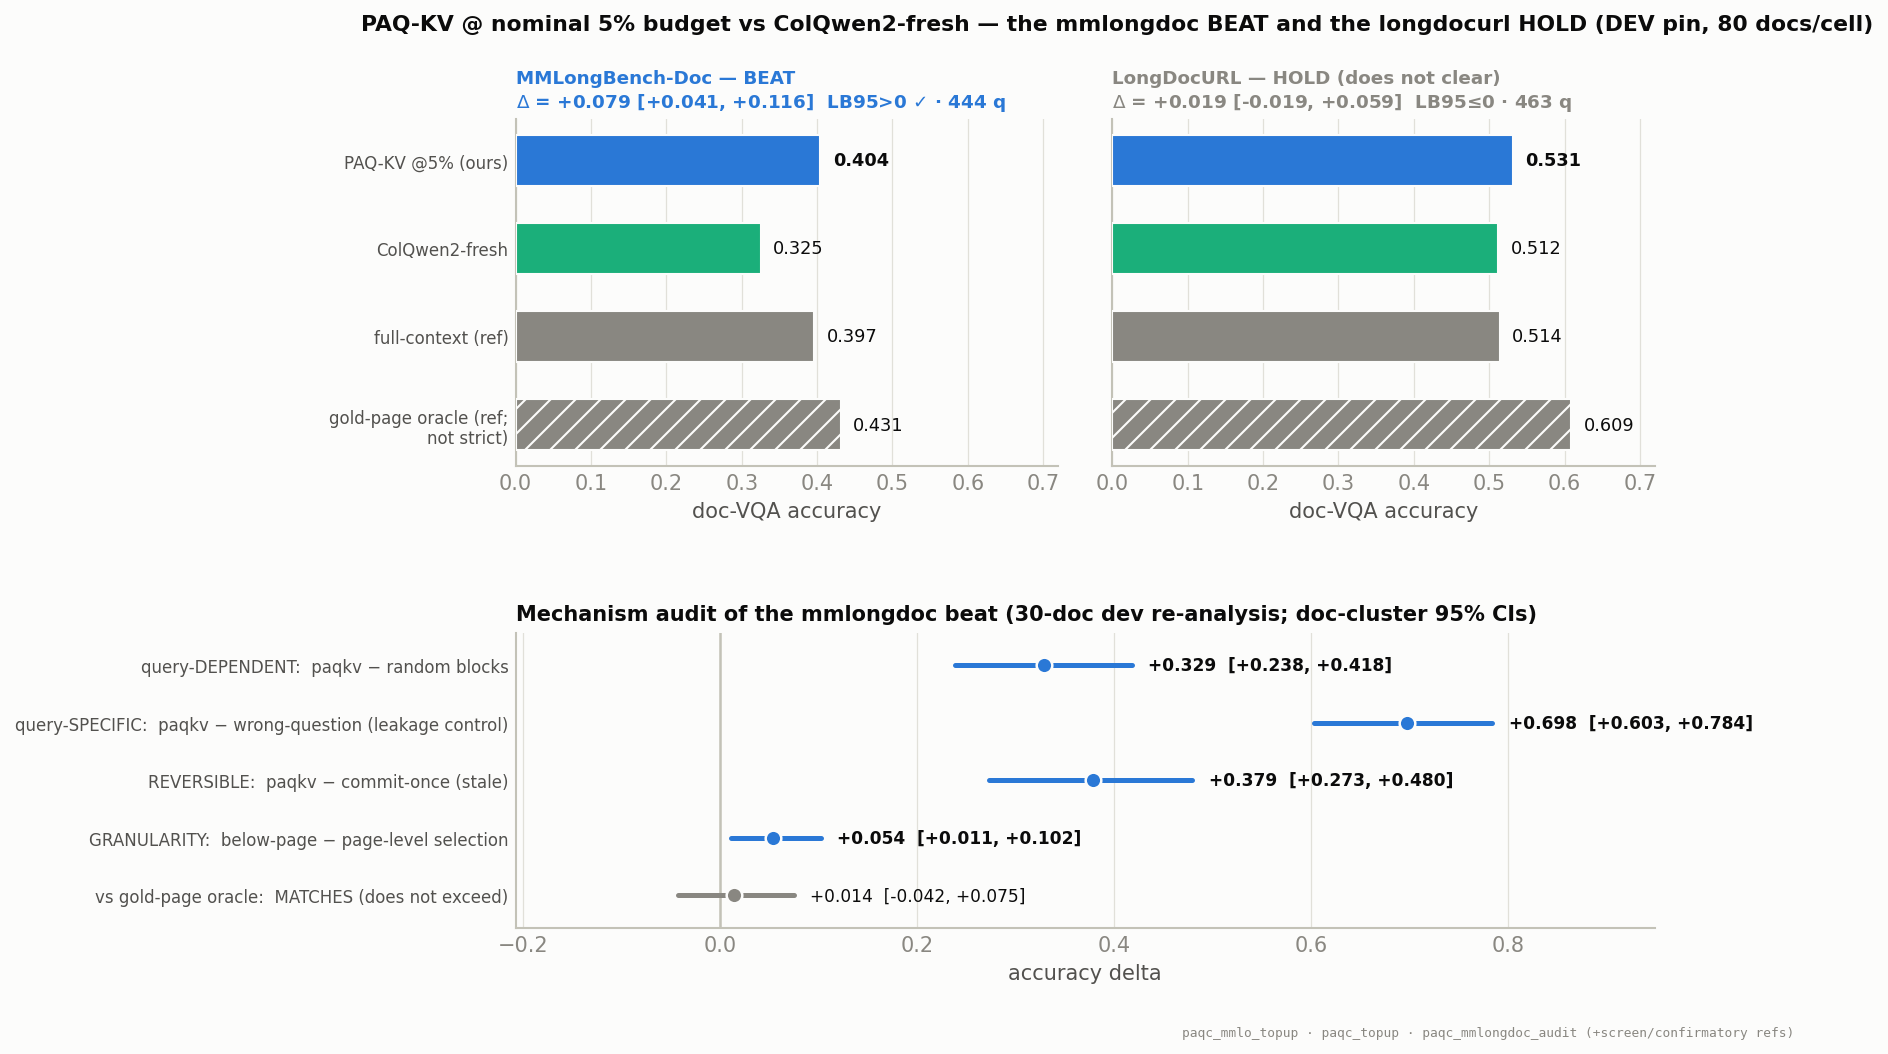
\includegraphics[width=0.86\textwidth]{fig_k_paqkv_results_light.png}
\caption{The results panel. \textbf{Top:} \paqc{}@5\% vs.\ ColQwen2-fresh with the full-context and gold-page-oracle references, per cell, with document-cluster CIs: the MMLongBench-Doc beat clears ($\lb=+0.041$); LongDocURL holds ($\lb=-0.019$). \textbf{Bottom:} the mechanism audit of the beat (30-document development re-analysis): selection is query-dependent, query-specific (the wrong-question collapse rules out leakage), reversible, and below-page ${>}$ page-level; against the gold-page oracle \paqc{} \emph{matches}---the CI straddles zero, and we do not claim to exceed it.}
\label{fig:paqkvresults}
\end{figure*}

\paragraph{The result.} At 80 documents / 444 queries, \paqc{}@5\% scores $0.404$ vs.\ ColQwen2-fresh $0.325$: $+0.079$, $\lb=+0.041$---the pre-frozen per-cell bar clears with margin (Table~\ref{tab:paqkv}, Figure~\ref{fig:paqkvresults}). Attending to a twentieth of the context, \paqc{} \emph{matches} full context ($+0.009$ $[-0.022,+0.040]$) and \emph{matches} the gold-page oracle ($-0.026$ $[-0.059,+0.008]$).

\paragraph{Correction of an earlier over-claim.} An earlier internal draft said \paqc{} ``beats the gold-page oracle'' on this cell. The adversarial audit showed that to be a small-sample artifact: the contrast straddles zero at both scales (30-document $+0.014$ $[-0.042,+0.075]$; 80-document $-0.026$ $[-0.059,+0.008]$). The correct statement---still the striking one---is that \paqc{} \textbf{matches the gold-page oracle at a ${\sim}5\%$ budget}: parity at a fraction of the budget, not a beat of the oracle. The oracle is defined identically on both cells and was pre-registered as \emph{not} a strict ceiling.

\paragraph{The mechanism audit.} The beat survives every mechanistic adversarial check (30-document development data, document-cluster CIs; Figure~\ref{fig:paqkvresults}, bottom):
\begin{itemize}
\item \textbf{query-dependent}: \paqc{} $-$ random-block selection $= +0.329$ $[+0.238,+0.418]$;
\item \textbf{query-specific}: \paqc{} $-$ wrong-question selection (select with a \emph{different}, disjoint-gold query's blocks; decode the true question) $= +0.698$ $[+0.603,+0.784]$---the collapse rules out leakage and query-invariant shortcuts;
\item \textbf{reversible}: \paqc{} $-$ commit-once $= +0.379$ $[+0.273,+0.480]$;
\item \textbf{granularity}: below-page $-$ page-level selection at matched budget $= +0.054$ $[+0.011,+0.102]$---the granularity itself, not just query-awareness, carries accuracy on this cell.
\end{itemize}

\paragraph{Caveats, kept visible.} The audit contrasts re-analyze 30-document development data (the beat itself is at 80 documents; the audit's named residual risk---sample size---was retired by the top-up). The screen's budget-curve monotonicity gate failed on this cell ($0.398$ at 10\% vs.\ $0.402$ at 5\%: selection quality, not budget, moves this cell; disclosed). And everything is development-pin evidence pending the sealed one-touch.

\subsection{LongDocURL: A Characterized Limitation}\label{sec:results-longdocurl}

At 80 documents / 463 queries, \paqc{}@5\% scores $0.531$ vs.\ ColQwen2-fresh $0.512$: $+0.019$, $\lb=-0.019$---a positive point estimate that does \textbf{not} clear the pre-frozen bar. The mechanism checks (query dependence, reversibility) clear on this cell too; what is missing is the margin. A re-analysis of the executed rows characterizes why:
\begin{enumerate}
\item \textbf{The significance bar is ${\approx}$twice the observed delta.} At 80 documents the per-document delta s.d.\ is $0.173$, giving a planning-level bootstrap s.e.\ of ${\approx}0.020$: an observed $\lb>0$ needs $\Delta \gtrsim +0.039$. (This symmetric-normal figure is a planning approximation for a percentile bootstrap, used as a compass, not a gate.)
\item \textbf{Only ${\approx}10\%$ of queries are selection-capturable.} Joint failure taxonomy over the 463 rows: $48.4\%$ are answered under both \paqc{} and the gold-page oracle; $39.1\%$ \textbf{fail under both}---zero even when the reader is handed exactly the gold pages at native resolution, so no selection method of any kind can rescue them (a \emph{reader-conversion wall}, ${\approx}41\%$ of the cell counting the oracle-fail mass); $10.4\%$ are oracle-right/\paqc{}-wrong (the entire selection-capturable pool, worth $+0.05$ net if captured perfectly); $2.2\%$ have \paqc{} beating the oracle.
\item \textbf{Resolution is not the lever.} Native page resolution is below the prefill per-page token cap for 79/80 documents (median native/cap $=0.50$): the prefill and the oracle already see native resolution.
\item \textbf{Large documents are a low-leverage dead zone.} Per-document mean(\paqc{} $-$ ColQwen2): $+0.064$ on the smaller half (25--44 pages) vs.\ $-0.005$ on the larger half (44--102 pages), where every arm is flat (${\approx}0.48$ at any budget) and even the native-resolution gold-page oracle reaches only $0.534$.
\item \textbf{Pure-selection ceilings are at best knife-edge.} Measured per-query oracle-chooser unions cap at or below the bar: best-of-budgets $+0.023$; tile${\vee}$stripe geometry $+0.024$; a two-scorer union (diffuse${\vee}$sharp, \S\ref{sec:results-negatives}) clears only at $\lb=+0.003$---and requires an \emph{undeployable} per-query oracle chooser. The only measured lever with comfortable headroom is a \paqc{}${\,\cup\,}$ColQwen2 combination (union oracle $\lb=+0.061$), which we exclude: a retriever-in-the-loop ensemble is not a standalone selection method, and ``a hybrid system beats standalone ColQwen2'' is a different claim.
\end{enumerate}
In short: on LongDocURL the binding constraint is the reader's evidence-to-answer conversion and the cell's variance structure, not selection quality. The two cells sharpen into a two-regime statement: below-page reversible selection wins on \textbf{dispersed-evidence} documents (MMLongBench-Doc) but not on \textbf{conversion-bound} ones (LongDocURL), where the wall sits past selection entirely.

\subsection{Negative Ablations, at Full Prominence}\label{sec:results-negatives}

\paragraph{Externally learned per-head mixture: STOP.} To remove benchmark supervision from selection, we trained a logistic per-head mixture over all $36{\times}32=1{,}152$ (layer, head) question$\to$page attention channels, contrastively, on off-benchmark provenance-checked data (every training page perceptually hashed against all 40{,}442 benchmark page images), with every design choice selected on external development data. The pre-frozen transfer gate failed: mixture gold-page recall $0.652$/$0.594$ vs.\ $0.676$/$0.616$ for a \emph{single} externally selected head; pooled mixture $-$ single $=-0.023$ $[-0.037,-0.008]$ (907 queries)---the $1{,}152$-weight mixture overfits its training distribution, and spreading weight over many heads loses to committing to one good head on transfer. The byproduct is real: the best zero-benchmark-contact head, \textbf{L21.H18}, coincides with the expert layer found independently by benchmark-supervised cross-validation---evidence the expert head is a property of the model, not of the benchmarks. No adapter training was run beyond this gate.

\paragraph{Sharp expert head as block scorer: NO-GO.} Swapping \paqc{}'s diffuse mean-attention block scorer (V0) for the transfer-validated sharp head L21.H18 (V1) failed all three pre-frozen conditions: on LongDocURL, V1 nudges the point estimate ($0.531 \to 0.536$; V1 $-$ ColQwen2 $= +0.024$ $[-0.012,+0.066]$) but does not separate from V0 ($\lb(\mathrm{V1}-\mathrm{V0}) = -0.011$, n.s.); on MMLongBench-Doc it \emph{hurts} ($0.402 \to 0.381$ on the screen documents). The lesson generalizes a recurring theme of this program: \textbf{recall-optimized selection is not accuracy-optimized selection}---a sharper, retrieval-style scorer concentrates budget on what looks relevant to a ranking objective and loses the contextual slack the diffuse scorer keeps.

\subsection{Why Below Page: The Page-Level History}\label{sec:results-pagelevel}
The program's page-level lineage is retained in full (Appendix~\ref{app:pagelevel}) because it motivates the method. A coarse-preview page router with a full-resolution re-read \emph{loses} to ColQwen2-fresh by ${\approx}10$ accuracy points at matched page budget (pooled $-0.099$ $[-0.129,-0.072]$); upgrading its scorer to a cross-validated expert attention head---CAPS's technique \citep{zhu2026caps}---recovers the entire gap to \emph{parity} ($+0.006$/$+0.028$ per cell; pooled $\lb=-0.000$), not past it, under a pre-registered non-inferiority protocol with an adversarial missingness analysis that erased an initially rosier complete-case edge. Page-level attention selection is published (CAPS), and page-level accuracy saturates at retriever parity; both facts pushed the program below page granularity, where the beat of \S\ref{sec:results-mmlo} lives.

\subsection{Efficiency: Accounting Only, No Claim}\label{sec:results-efficiency}
No latency/VRAM/throughput table exists yet, so we make \textbf{no efficiency claim}. For orientation only: after the one prefill, a \paqc{} query costs one short question forward plus a masked decode over an already-resident cache, whereas ColQwen2 still pays a per-query prefill of the re-read selected pages and CAPS re-forwards every page per query. A measured table (cold/warm start, co-resident vs.\ sequential retriever, index bytes per page, queries-per-document break-even) is required before any such claim.

\section{Limitations}\label{sec:limitations}
\begin{itemize}
\item \textbf{Development-pin evidence only.} Every \paqc{} number comes from the reused 80-document development pin; the sealed 73/45 one-touch final has not run, and until it does the MMLongBench-Doc beat is development-grade evidence. The sealed MMLongBench cell (244 queries / 45 documents) sits below the program's 250-query power floor, so the sealed confirmation needs the effect to hold at slightly reduced power.
\item \textbf{One cell of two.} The beat is scoped to the dispersed-evidence regime; LongDocURL is a characterized hold, not a win.
\item \textbf{Single reader.} All results are a Qwen3-VL-8B case study; generalization to other VLMs is untested.
\item \textbf{Budget semantics.} The \paqc{} budget is a nominal 5\% decode-attention budget (realized ${\approx}5.9$--$6.0\%$) with block K/V computed under full-document prefill context---Quest/SnapKV claim semantics, not a matched-token prefill comparison.
\item \textbf{Audit scale and provenance.} The mechanism-audit contrasts re-analyze 30-document development data; the LongDocURL full-context reference in Table~\ref{tab:paqkv} is a 30-document screen value (disclosed).
\item \textbf{No efficiency claim} (\S\ref{sec:results-efficiency}); the mask route is the accuracy path and physical gathering is future work.
\item \textbf{Base-model ceiling.} $35.1\%$ of confirmatory queries are oracle-unanswerable, deflating absolute numbers for every arm; the query-blind eviction arms are disclosed proxies we claim nothing against.
\item \textbf{Protocol residues.} The commit-once aggregate uses the first $M{=}\min(3,k)$ queries in frozen arrival order (order-permutation and $M$-sensitivity checks remain to be run; the order-free static partially covers this), and the page-level confirmatory run predates the cache fix (\S\ref{sec:integrity})---its isolation \emph{contrasts} were verified robust, but its absolute fresh-arm levels carry ${\approx}0.04$ inflation on the 24-document check.
\end{itemize}

\section{Conclusion}
\paqc{} turns a frozen VLM's own KV cache into a reversible, query-conditioned evidence store: prefill once, then per query re-select below-page blocks and decode under a restricted-attention mask over the intact cache. Reversibility---re-selection beating commit-once---is confirmed on both cells, across scorers, and across granularities; on dispersed-evidence long-document VQA the full method beats a state-of-the-art trained visual retriever at matched budget while matching the gold-page oracle at ${\sim}5\%$ of context, with the mechanism adversarially audited. Where it does not beat the retriever, we say so and show why the cell resists all selection methods. The sealed held-out evaluation is the single remaining step for mandate-grade evidence, and the two-regime characterization (dispersed-evidence vs.\ conversion-bound) is, we believe, the right frame for where below-page reversible selection helps.

\bibliography{references}

\appendix

\section{Full Executed Panel}\label{app:panel}

Table~\ref{tab:panel} reports every executed arm at the gate budget on the confirmatory pin. The query-blind eviction family sits at or below random gold-page recall on these cells---the anti-strawman record: beating it is visibly not the claim. Secondary pooled statistics: the fresh page-level selector beats the best family arm (SnapKV-stale) with min-over-family $\lb = +0.202$; fresh $-$ SnapKV-fresh $= +0.094$ $[+0.069,+0.122]$; fresh $-$ oracle $= -0.199$ $[-0.239,-0.161]$. Gold-page recall at $b{=}5\%$ (LongDocURL / MMLongBench-Doc): fresh page selector $0.494/0.443$; gold-informed static $0.381/0.373$; same-scorer commit-once $0.137/0.148$; ColQwen2-fresh $0.664/0.536$.

\begin{table}[t]
\centering\small
\setlength{\tabcolsep}{3.5pt}% permitted narrowing (AAAI kit)
\begin{tabular}{llcc}
\toprule
Group & Arm & LDU & MMLB \\
\midrule
\multirow{2}{*}{ours (page level)}
 & \paq{} (fresh) & \textbf{0.386} & \textbf{0.258} \\
 & attn\_max (alt-agg) & 0.337 & 0.152 \\
\midrule
\multirow{2}{*}{isolation}
 & same-scorer commit-once & 0.128 & 0.095 \\
 & gold-informed static & 0.278 & 0.154 \\
\midrule
\multirow{3}{*}{retrieval}
 & ColQwen2-fresh & 0.512 & 0.328 \\
 & ColQwen2-stale & 0.216 & 0.138 \\
 & CLIP-fresh & 0.155 & 0.164 \\
\midrule
\multirow{3}{*}{reference}
 & SnapKV-fresh & 0.298 & 0.157 \\
 & full-context & 0.546 & 0.397 \\
 & oracle-evidence & 0.609 & 0.431 \\
\midrule
\multirow{7}{*}{query-blind}
 & SnapKV-stale & 0.083 & 0.074 \\
 & H2O & 0.045 & 0.039 \\
 & FastV (proxy) & 0.045 & 0.031 \\
 & LOOK-M ($\to$H2O) & 0.045 & 0.039 \\
 & KVzip (proxy) & 0.047 & 0.048 \\
 & random & 0.068 & 0.022 \\
 & truncation & 0.033 & 0.041 \\
\bottomrule
\end{tabular}
\caption{Every executed arm, accuracy at $b{=}5\%$, per cell (LDU = LongDocURL, MMLB = MMLongBench-Doc), on the confirmatory pin. Query-aware arms marked fresh re-select per query; stale arms commit once per document.}
\label{tab:panel}
\end{table}

\section{The Page-Level History in Detail}\label{app:pagelevel}

\paragraph{The page router (\paq{} v1).} Pages are rendered at coarse resolution (${\approx}3.5$K visual tokens total, i.e.\ ${\approx}70$ tokens/page on a 50-page document) and prefilled once; per query, the question rows' attention (mean over heads, layers, and question tokens) scores pages; the top pages at budget $b$ are re-rendered at full resolution and read. This is page routing, not KV compression, and it claims no memory savings.

\paragraph{The retrieval loss.} At $b=5\%$, ColQwen2-fresh scores $0.512$/$0.328$ vs.\ \paq{} $0.385$/$0.258$: pooled $-0.099$ $[-0.129,-0.072]$---an ${\approx}10$-point loss that holds on every stratum examined (Figure~\ref{fig:retrieval}). Gold-page recall is consistent with a coverage contribution: ColQwen2-fresh $0.664$/$0.536$ vs.\ \paq{} $0.494$/$0.443$. Both scorers collapse when committed once (ColQwen2 stale $0.216$/$0.138$), reproducing the reversibility pattern with a second scorer family.

\begin{figure}[t]
\centering
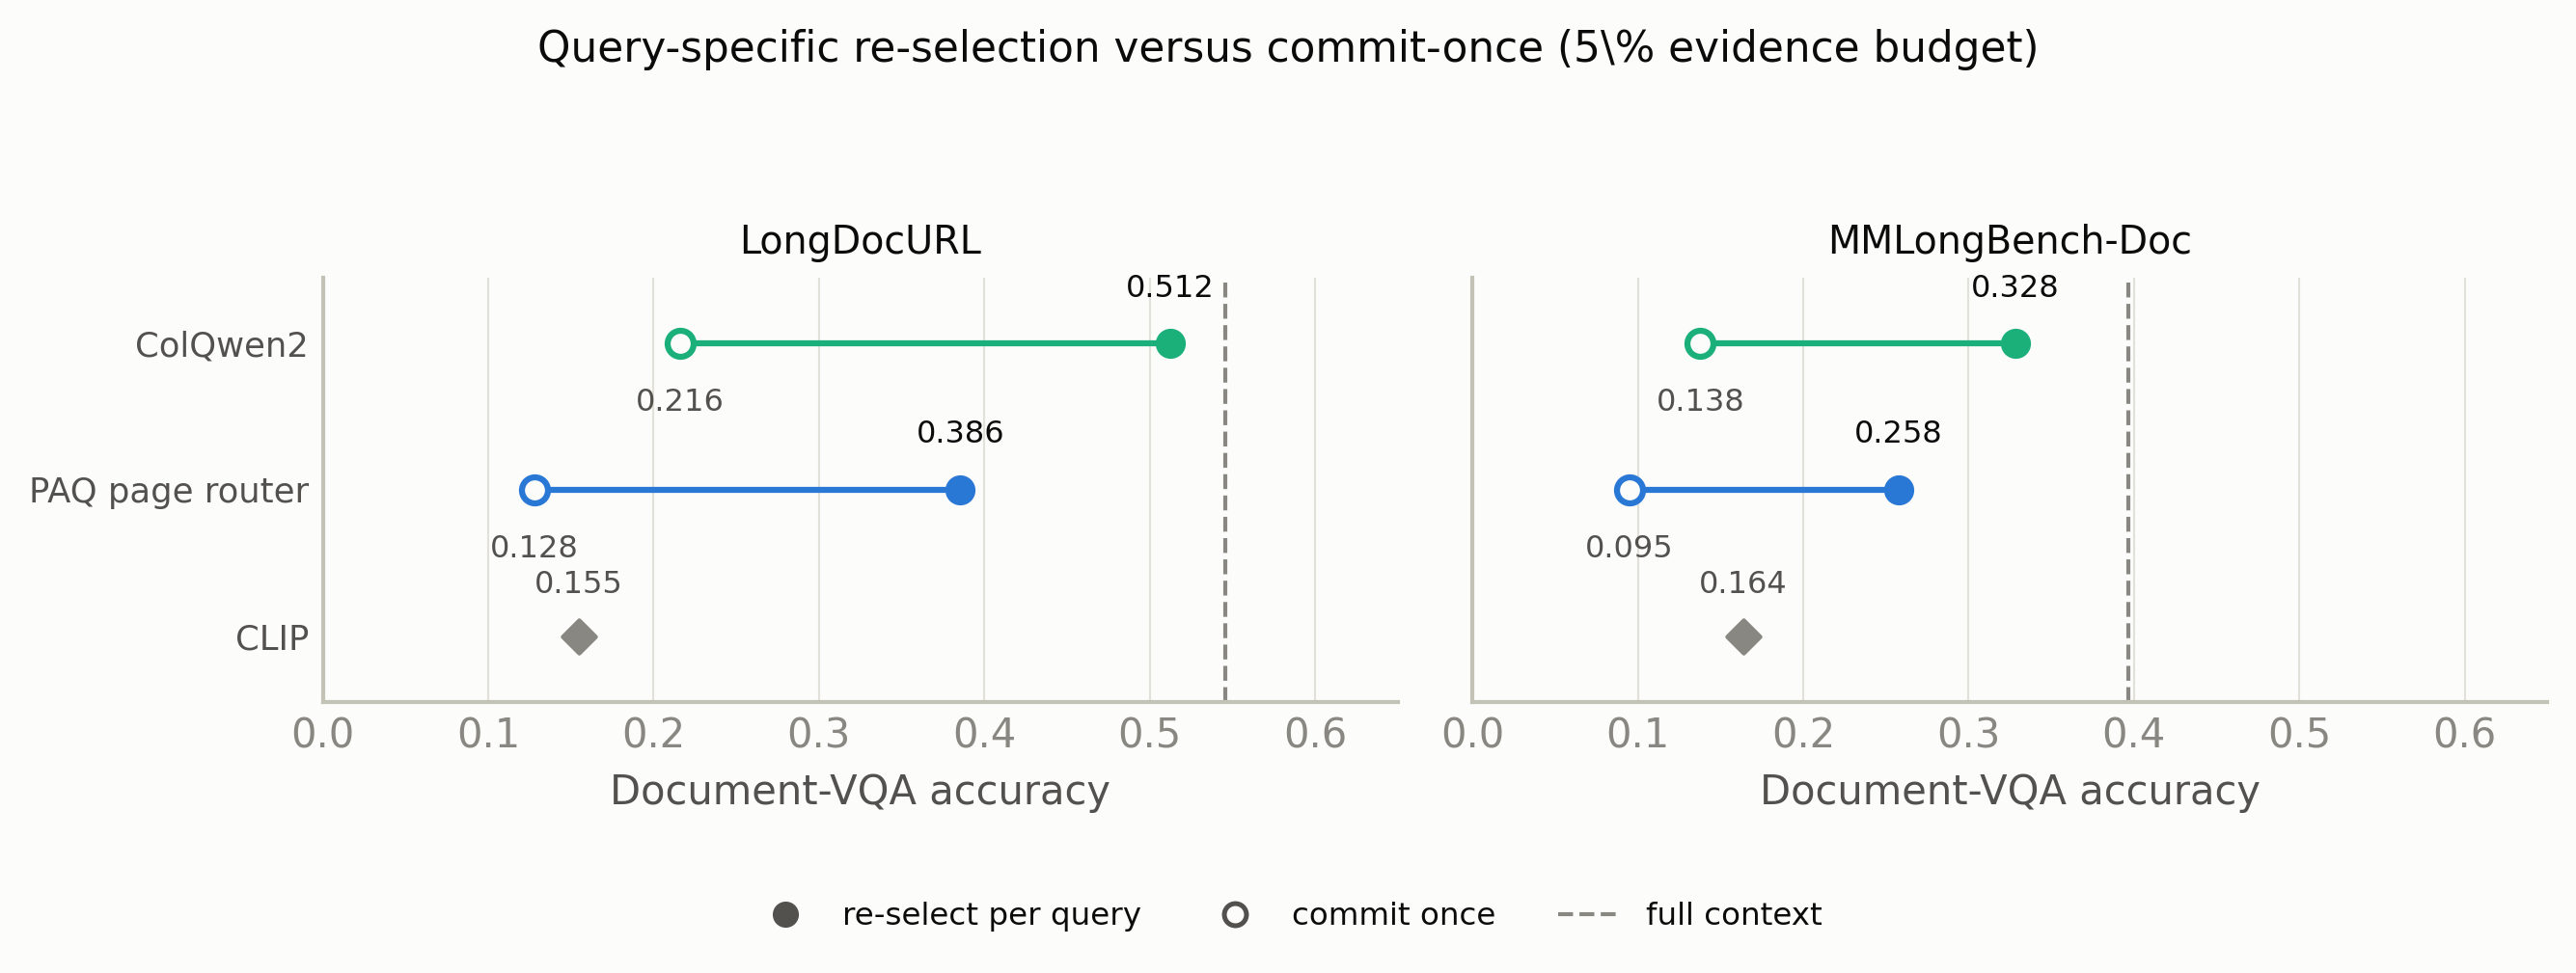
\includegraphics[width=\columnwidth]{fig_e_retrieval_reversal_light.png}
\caption{The two honest facts of the page-level history, per cell: (i) ColQwen2-fresh beats the page-level attention router (the ${\approx}10$-point loss); (ii) \emph{both} scorers collapse when committed once---reversibility is a general property of the multi-query regime, not scorer-specific.}
\label{fig:retrieval}
\end{figure}

\paragraph{\paqt{}: expert-head recall and the parity read-eval.} Scoring with a single expert (layer, head) chosen by held-out-document cross-validation---CAPS's technique---lifts held-out gold-page recall@5\% to $0.683$ ($n{=}451$) / $0.626$ ($n{=}425$), meeting or exceeding ColQwen2's in-harness $0.664$/$0.536$; mean aggregation at higher scoring resolution moves almost nothing ($0.494/0.443 \to 0.500/0.452$), so the head, not resolution, is the lever. All selected fold heads sit in layer 21. The pre-registered accuracy read-eval (bars frozen before the run; same reader, render policy, and scorer as the cached baseline rows; only the selected page set differs) lands at \textbf{parity}: \paqt{} $0.518$/$0.357$ vs.\ ColQwen2-fresh $0.512$/$0.328$; deltas $+0.006$ $[-0.018,+0.030]$ and $+0.028$ $[+0.001,+0.055]$; pooled $+0.017$ $[-0.000,+0.035]$---non-inferior under the frozen $\lb > -0.03$ margin on both cells, but not the pre-registered beat (all $\lb>0$), and we do not present the razor's-edge per-cell interval as a win. The initially better-looking complete-case verdict (pooled $+0.023$, $\lb=+0.005$) was \emph{blocked} in review for informative missingness---the ${\approx}4\%$ of queries whose high-resolution scoring ran out of memory had cached baseline accuracy $0.62$, far above the cell means---and a conservative reduced-resolution recovery of 31/35 missing rows (degrading only the \paqt{} arm, never the baseline) erased the pooled edge. Two caveats carry over: head selection is cross-validated \emph{benchmark-supervised} model selection (not zero-shot; the externally selected L21.H18 of the STOP ablation later removed this caveat from the head's existence, not from its benchmark-tuned use), and the expert-head technique is CAPS's---the residual novelty at page level is only the amortized one-prefill-many-queries architecture.

\section{Additional Reversibility Detail}\label{app:reversibility}

\begin{figure}[t]
\centering
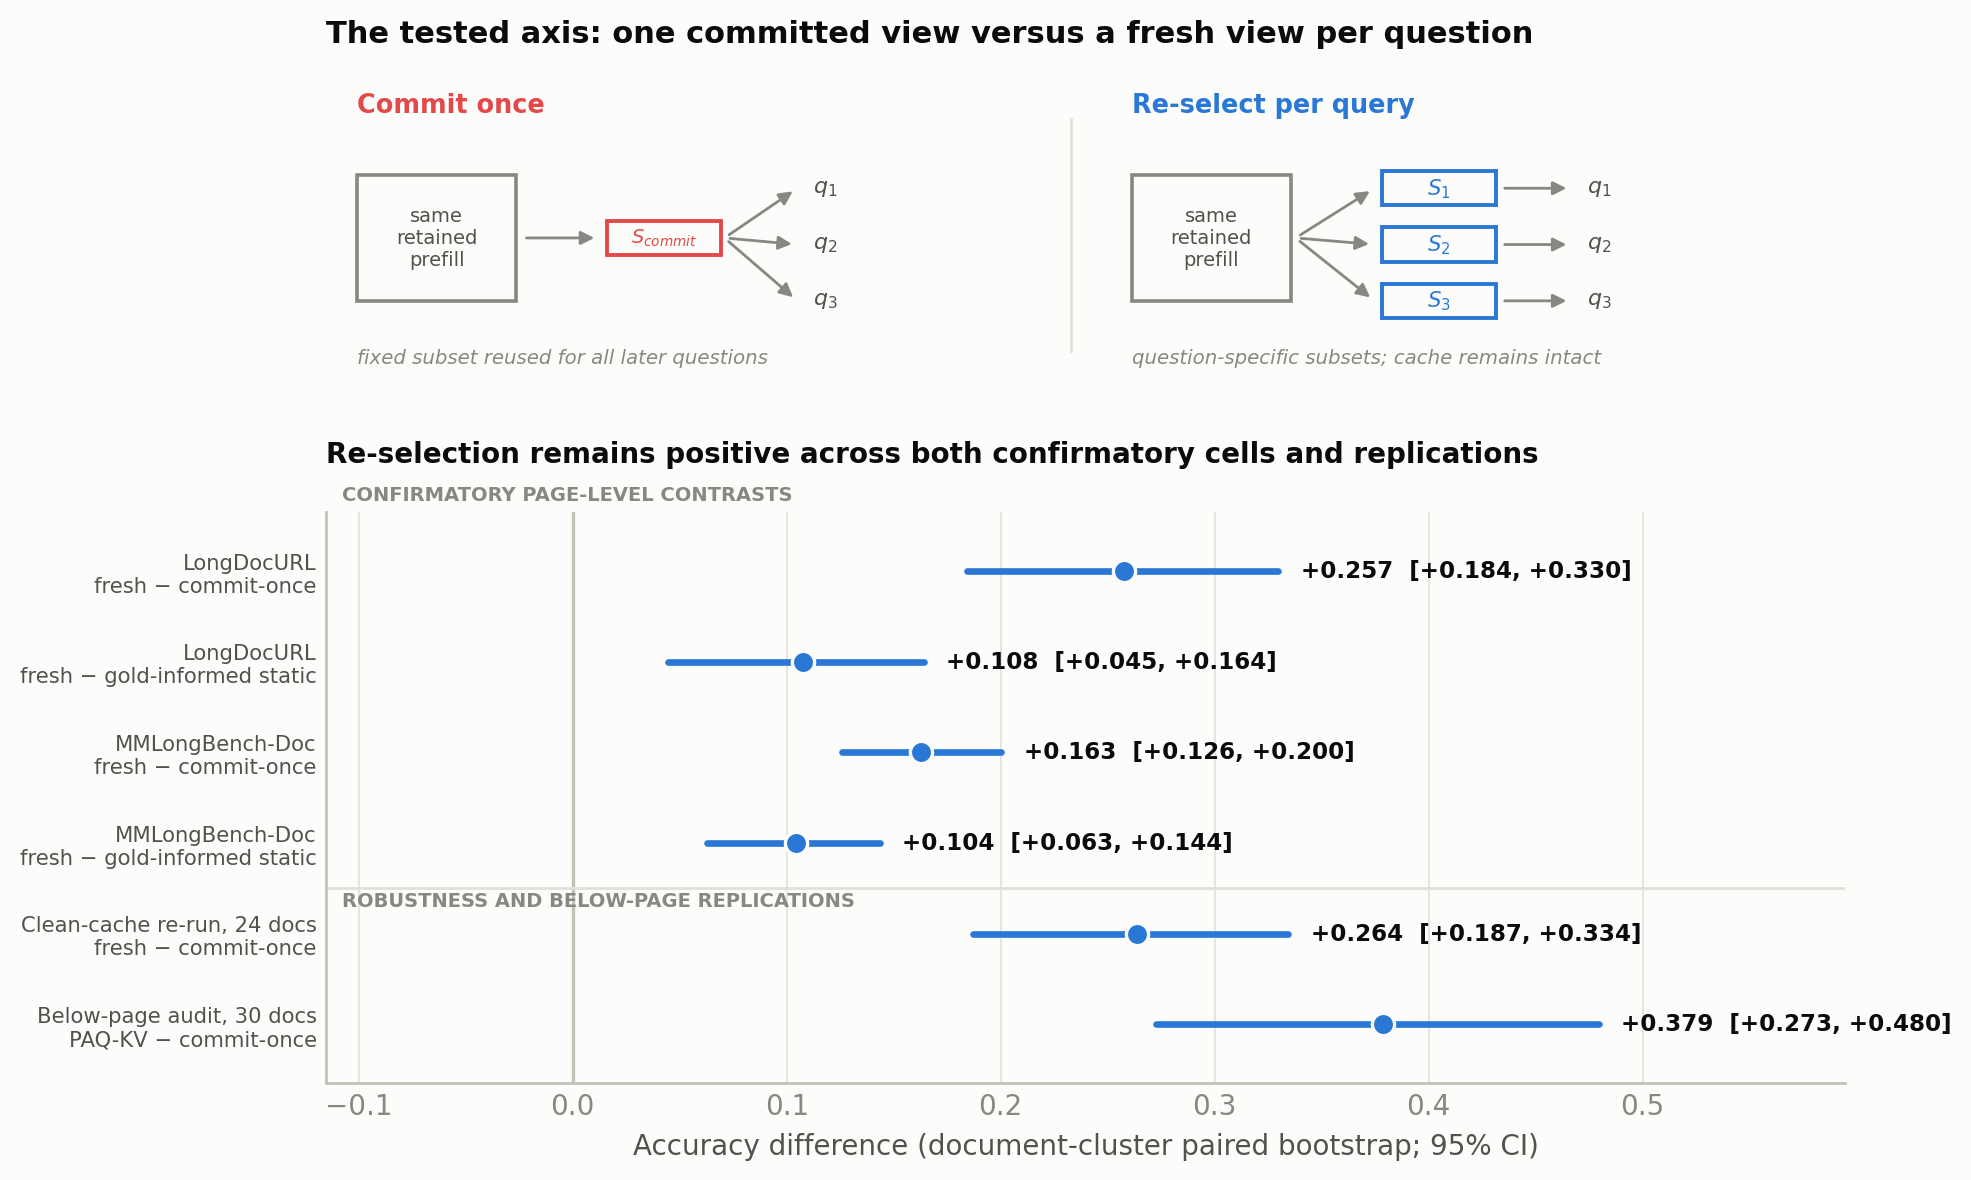
\includegraphics[width=\columnwidth]{fig_j_reversibility_light.png}
\caption{Reversibility---the tested axis. \textbf{Top:} a commit-once deployment reuses one subset for every question and goes stale; re-selection re-derives the subset per query from the same retained prefill. \textbf{Bottom:} the isolation protocol across granularities: the confirmatory page-level contrasts, the clean re-run after the cache fix, and the block-level \paqc{} contrast. Every interval clears zero.}
\label{fig:reversibility}
\end{figure}

\begin{figure}[t]
\centering
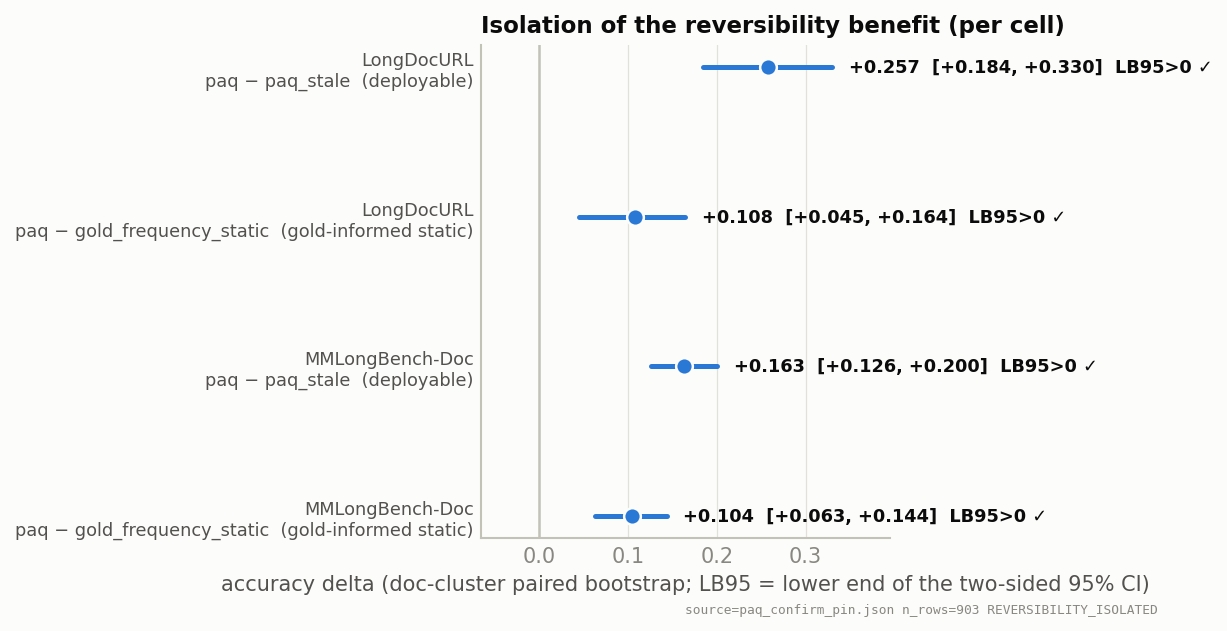
\includegraphics[width=\columnwidth]{fig_b_isolation_forest_light.png}
\caption{Per-cell forest of the two page-level isolation contrasts at $b=5\%$. Intervals are document-clustered two-sided 95\% CIs; all four exclude zero.}
\label{fig:forest}
\end{figure}

Figures~\ref{fig:reversibility} and~\ref{fig:forest} show the reversibility axis schematically and the per-cell forest of the confirmatory isolation contrasts. Additional pre-registered analyses: (i) \emph{answerable subset} (secondary; conditions on a model outcome): on queries where oracle-evidence scores exactly 1 ($n=407$), fresh $0.583$ vs.\ commit-once $0.182$ ($+0.395$ $[+0.324,+0.460]$) and vs.\ the static $0.382$ ($+0.204$ $[+0.135,+0.266]$); (ii) \emph{missingness}: 4 of 907 vision queries are missing due to a per-document timeout; worst-case imputation in either direction leaves the gate verdict unchanged; (iii) \emph{budget curves}: the fresh selector dominates both static comparators at every budget in $\{2.5, 5, 10\}\%$ on both cells; at $b=10\%$ on LongDocURL it reaches $0.518$ vs.\ full-context $0.546$---reading 10\% of pages recovers ${\approx}95\%$ of full-context accuracy on that cell (not on MMLongBench-Doc: $0.317$ vs.\ $0.397$).

\paragraph{Cache-pollution quantification.} The in-place cache bug of the main text was quantified before being fixed: on a 6-documents-per-cell blast-radius diagnostic (87 query-rows), the bug inflates gold-page recall by ${\approx}+0.05$ for a fixed scoring head and shifts selections (mean top-$B$ Jaccard clean vs.\ polluted $0.82$, drifting from $1.00$ at $q_0$ to $0.61$ at $q_6$), as expected for cumulative contamination. The recall gate behind the \paqt{} numbers was regenerated clean before any accuracy read (clean held-out expert recall $0.683$/$0.626$ vs.\ polluted $0.674$/$0.628$), and the clean cross-validation picks a more robust head. Absolute fresh-arm accuracy in the pre-fix confirmatory carries ${\approx}0.04$ inflation (clean $-$ polluted $-0.041$ $[-0.077,-0.003]$ on the 24-document check); the isolation contrasts cancel the bug and stand.

\section{Reproducibility and Protocol Notes}\label{app:repro}

\paragraph{Pre-registration discipline.} Every gate in this program was frozen (bars, comparators, budgets, imputation policy) before its run: the two-comparator isolation gate; the \paqt{} read-eval bars (non-inferiority/beat/inferior margins, per-cell power floors, adversarial missingness imputation); the per-head-mixture transfer gate; the \paqc{} decode-identity kill criterion, screen gates, per-cell beat bars, and the sharp-scorer (V1) gate. Two early positives did not survive adversarial review and were retracted before this draft: a first isolation gate against the eviction family (invalidated by a weak-static artifact and replaced by the two-comparator gate), and the ``beats the gold-page oracle'' phrasing (corrected to ``matches'' at power). The commitment-pressure mechanism hypothesis failed its formal test and is reported as exploratory.

\paragraph{Instrumentation.} All significance statements use one instrument: the document-cluster paired bootstrap (10{,}000 draws, seed 0, percentile intervals; equal-cell pooling), unit-tested alongside the gate and pairing logic. Evaluation pins are sha-256 checksummed and byte-verified before use; the screen pin is a strict prefix of the confirmatory pin, and independent-extension analyses use the 50 new documents per cell only. Figures are generated from the verdict artifacts by a single script; nothing is hand-entered. Per-query, per-arm rows, frozen-bar metadata, verdict files, and the adversarial review trail are retained and will be released with the code.

\paragraph{Sealed one-touch protocol.} The 80-document confirmatory pin has been reused across this program and is therefore development-only. The fresh sealed set (73 LongDocURL documents / 433 queries; 45 MMLongBench-Doc documents / 244 queries; zero overlap with the pin) is reserved for a single final evaluation: the baseline will be run on it once, and the only mandate-grade claim this program will make is a scope-appropriate, adversarially imputed, document-clustered $\lb>0$ on that sealed set. It has not been evaluated; no number in this paper comes from it.

\end{document}
